\section*{Appendix D -- TRACE}

[Moving everything TRACE related here because it turns out we don't actually need it]



\paragraph{TRACE } How speech is perceived and understood has been a subject of much debate for a significant portion of psycholinguistics' history. Starting in the 1980s and persisting today, many researchers subscribe to what is known as the connectionist model of speech perception. Briefly, this model posits that speech perception is best understood as a hierarchical dynamical system in which aspects of the model are either self reinforcing or self inhibiting with feed-forward and feedback mechanisms. For example, hearing the phoneme \textbackslash h\textbackslash  \ as in ``hit" will ``feed-foward", cognitively activating words that begin with the \textbackslash h\textbackslash \  sound. These activated words then ``feedback" to the phoneme letter, inhibiting activation for competing phonemes such as \textbackslash b\textbackslash \ or \textbackslash t\textbackslash. In 1986, McClelland and Elman introduced the TRACE\footnote{TRACE doesn't stand for anything -- the name is a reference to ``the trace", a network structure for dynamically processing things in memory} model implementing theoretical considerations into a computer model \cite{elman1985speech}. Maybe useful here to discuss activation, sigmoidal shape, etc., 


\subsection{TRACE -- section}

I have a few issues with this section, and as I have fleshed out my reading and understanding of things, my intention with this section has changed. Originally, my hope was to show that non-linear functions fit with empirical saccade data would be a better match to what is predicted by TRACE than what is found using fixation data. This, however, seems to be the wrong thing to do. There is an apparently magnificent number of ways with which to transform TRACE activation data to probabilities of fixation, Neverminding the fact that the saccade curve is a fundamentally \textit{different} concept/mechanism than the proportion of fixations, calling into question the value of a direct comparison (though I'm not sure that this is really much of an issue, as none of these transformations had mechanics uniquely specific to the properties of fixations).

This general idea is related to an observation made earlier by Allopenna and friends, 

``It is important to note that although the TRACE simulations provided good fits to the behavioral data, the results should be taken as evidence in support of the class of continuous mapping models, rather than support for particular architectural assumptions made by TRACE."

Of course, this finds us in a bit of a circular loop -- Allopenna suggested that the consistency of evidence was used to support the assumptions of TRACE, and here we are suggesting TRACE as evidence for the saccade method. What seems more appropriate, then, is to demonstrate that there \textit{exist} transformations of TRACE data in which \textit{either} the saccade or fixation methods creates a better fit (as measured by $R^2$ or MISE). As such, it makes less sense to use TRACE to show which is ``better", but rather to use TRACE to demonstrate that what is estimated with the saccade method continues to be consistent with the continuous mapping model of lexical activation. Having established theoretical consistency, my argument for the saccade method will rest on what was presented in the previous section, namely the separation of saccades and fixations, and the problems illustrated with the added observation bias. 

As it is, I have a few sections here addressing high level concerns. How it should be precisely organized is up for debate, but the work itself should be largely finished.

Finally, I will note here without much other detail -- the entirety of this next section rests with the empirical and simulated data from McMurray 2010. For the empirical data, only N/TD subjects were used and for TRACE, only the 14 simulations with the default hyper-parameters from jTRACE. The specifics of data processing (less what I mention in relevant sections here) can be cast to the appendices

\subsection{On fitting saccade data}


I will go into more detail later on the precise transformations that I did to arrive at the empirical data from the raw data.  One key thing to note, however, is that rather than using the separate saccade data in the Access DB, I finished cleaning the fixation data and then transformed this to saccade data based on the start time of subsequent fixations. This helped address ambiguities that resulted from deciding which saccades to be included. For example, if we neglected to include any saccades that began before the onset of the audio signal, the first saccades recorded (generally) had a probability of fixating on the target of about 0.25, resulting in an empirical curve with a base parameter much closer to 0.2. Additionally, this first saccade often occured some time after onset, leading to virtually no observed data near $t = 0$. This was addressed by artificially setting the first saccade to have occurred at $t = 0$ with its direction set to match that of the matching fixation at the same time. After making this adjustment, the baseline of the saccade curve matched nearly that of the fixation curve, making the saccade curve more closely match the shape of the fixation curve.

Slightly more of an indulgence was how to treat the end of the saccade curves at each trial. Necessarily in all cases, following the last saccade, recorded fixations were constant until the end of the trial, drastically increasing the ``added observation" bias and resulting in a fixation curve with a peak much closer to 1.

On one hand, this could perhaps have been dealt with by addressing response times and making the appropriate adjustments. Or, far more simply (and with fewer researcher degrees of freedom), I simply added one last saccade to the end of each trial with it's location being that of the last fixation (typically the target object). The rest of the analysis does not depend on this decision in any fashion, and as the results are functionally the same, I elected to use the saccade curve with the inflated data. This most closely matches our expectation of the relation between the fixation and saccade curves and addresses (to some degree) the asymptotic behavior of the saccades which would otherwise be uncollected. A demonstration of these differences is given in Figure~\ref{fig:saccade_inflate}.

\begin{figure}
\centering
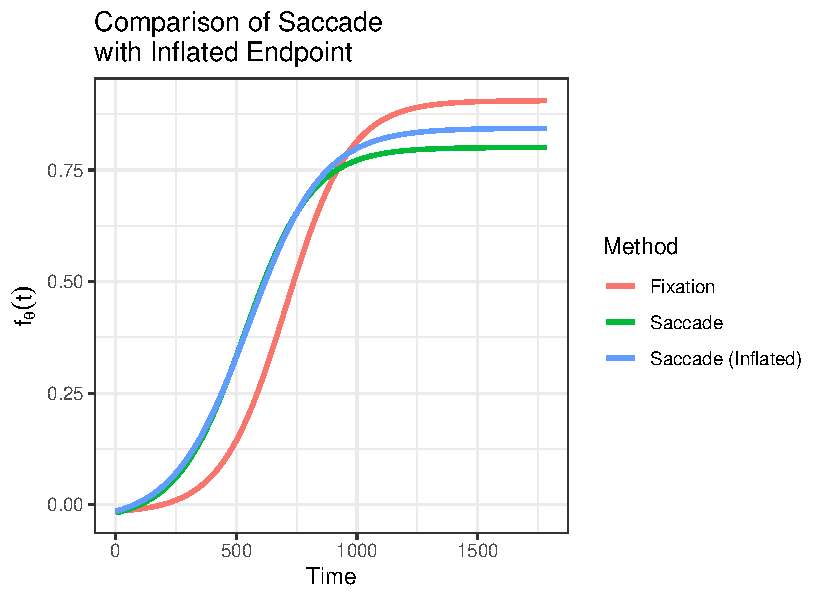
\includegraphics{sac_inflate_compare.pdf}
\caption{this is what happens when i inflate saccade with additional saccade at last endpoint}
\label{fig:saccade_inflate}
\end{figure}

\subsection{Transforming TRACE data}


My primary concern with the TRACE data is I am seemingly unable to reconcile it visually with what is presented in the 2010 SLI paper. Specifically, I never achieve a baseline near 0. I tried manipulating the temperature of the luce choice rule (LCR) with both constant factors and sigmoidal shapes with differing parameters; I also tried playing with some of the parameters from the scaling factor function.


Referring back to an email we exchanged 12/14/2022, you (you being theBob) gave me a list of adjustments to make to the scaling factor, including swapping the activation and crossover, as well as expanding the exponential term to include the entire denominator. I did this and confirmed that, as you had, the function goes from 0.0002 at maxact=-0.2 to .739 at maxact = .55. The issue, though, is that this is performed \textit{after} luce choice rule implemented. In that situation, the minimum activation observed is 0.25 rather than -0.2. This made me think that perhaps some other permutation of transformations would result in a curve starting closer to 0 and peaking nearer to .75 (for example, scaling the raw TRACE activations). In my collection of attempts, I never found anything to quite correct for this. It may be a bit much, but I have included plots of the TRACE data related to the target at different points in the transformation process to see how it changes. Maybe something in that will ring at bell. These are included in  Figure~\ref{fig:shades_of_trace}. 


An interesting aside, though -- if we do not make the adjustment to the saccade data where we anchor asymptotic behavior at 0/1, we get a saccade curve bearing less relation to the fixation curve, but with much higher agreement with the set of TRACE curves, in particular with regards to the baseline point and peak. Presumably with some tweaking, it could be made to match even more closely. This phenomenon is illustrated in Figure~\ref{fig:unadjusted_saccade_against_trace}

\begin{figure}[H]
  \centering
  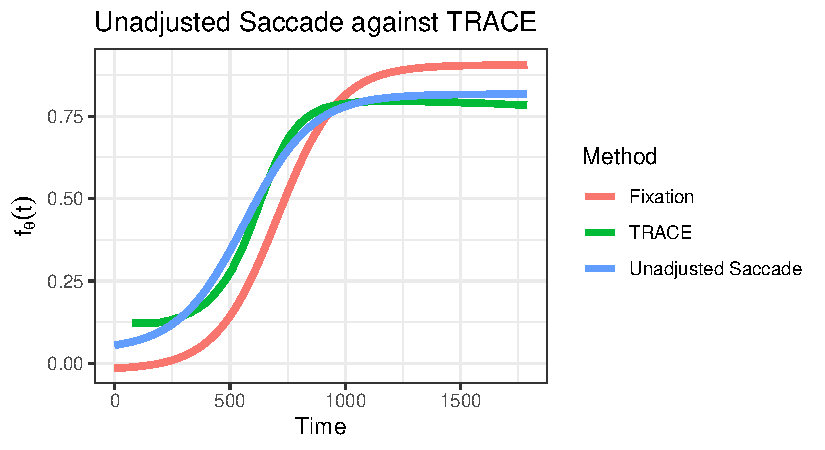
\includegraphics{unadjusted_sac_w_trace.pdf}
  \caption{Plot illustrating how the unadjusted saccade method (without anchoring at asymptotes) both matches more closely with the TRACE predictions (particularly near the baseline) while also taking on a far different shape than the fixation curve. This is in contrast to the Princess Bride simulations in which the distortion was minimal and the saccade curve appeared to be more of a horizontal shift}
  \label{fig:unadjusted_saccade_against_trace}
\end{figure}


\
\begin{figure}[H]
    \centering
    \subfigure[]{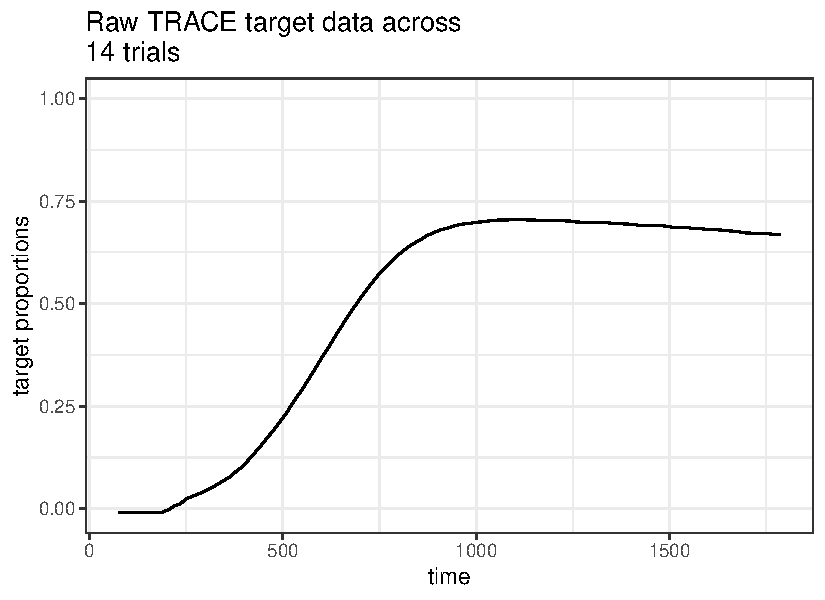
\includegraphics[width=0.45\textwidth]{TRACE_test/raw_trace.pdf}} 
    \subfigure[]{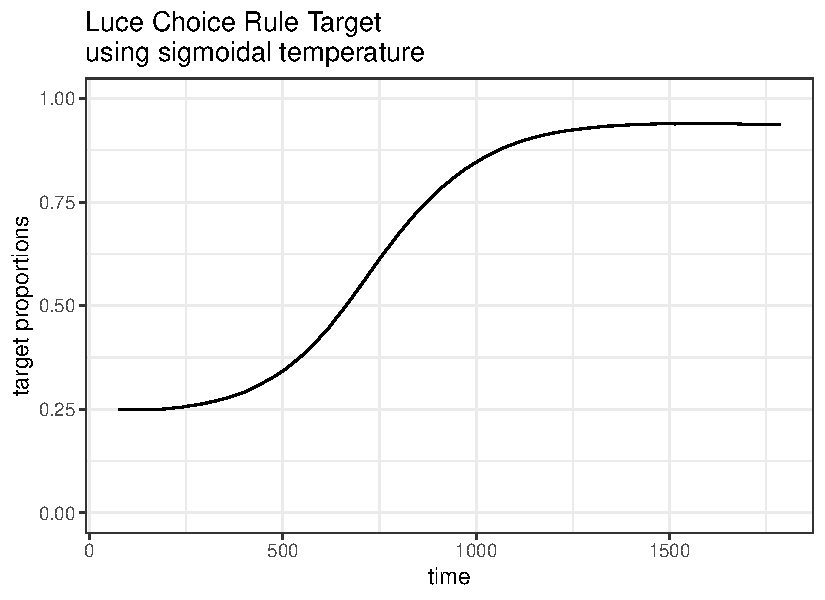
\includegraphics[width=0.45\textwidth]{TRACE_test/luce_choice.pdf}} 
    \subfigure[]{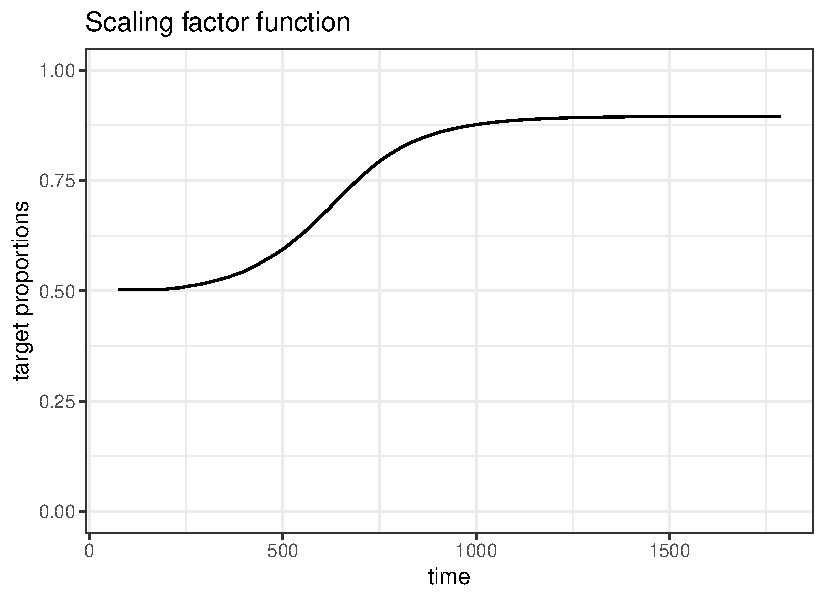
\includegraphics[width=0.45\textwidth]{TRACE_test/scaling_factor.pdf}}
    \subfigure[]{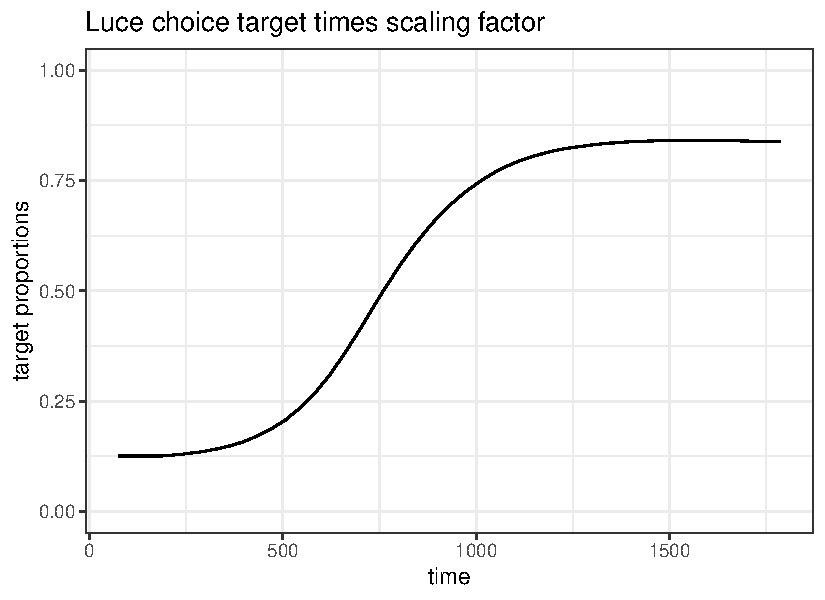
\includegraphics[width=0.45\textwidth]{TRACE_test/scaling_times_luce.pdf}}
    \subfigure[]{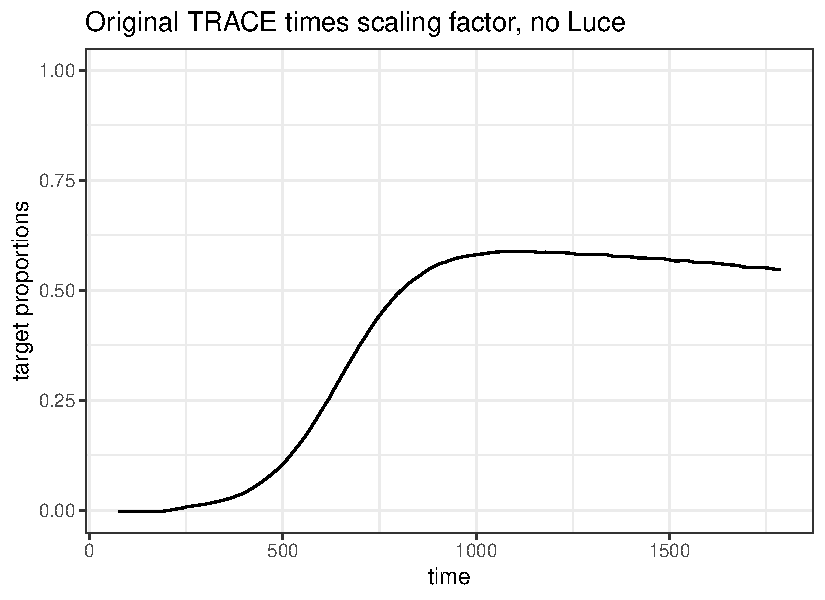
\includegraphics[width=0.45\textwidth]{TRACE_test/skipping_luce.pdf}}
    \begin{singlespace}
    \caption{(a) This is simply the raw TRACE data across the 14 simulations with standard parameters. (b) Transformation of TRACE activation using LCR with sigmoidal temperature. (c) Scaling factor function built on max activations \textit{after} performing LCR, using peak/baseline values from target object. (d) TRACE activations following LCR transformation and multiplying by scaling factor. This is what I have been using as model prediction of fixations, though note the baseline value being near 0.15. (e) Perhaps unnecessary, this is simply investigating TRACE activation by the scaling factor but without first conducting LCR. Note that none of these seem to have both the correct baseline and peak values} \end{singlespace}
\label{fig:shades_of_trace}
\end{figure}


\subsection{Comparisons}

Here is where I would suggest the consistency of the models. What I show here is a moderated version of this, namely I show that there are two transformations of TRACE (changing the parameters of the sigmoidal function for Luce choice rule, or the temperature directing the rate at which competitors are weeded out) that each match one or the other of the fixation/saccade curves better. As such, neither is superior in any sense, but both are in the realm of consistency.


\begin{figure}[H]
    \centering
    \subfigure[]{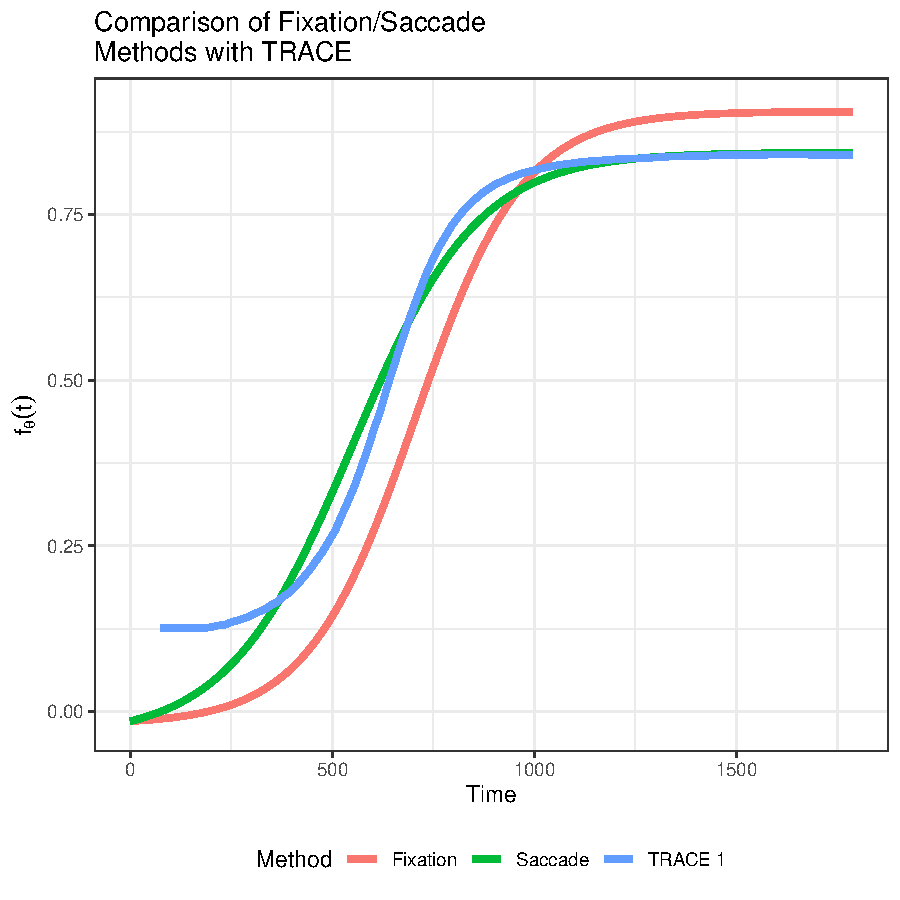
\includegraphics[width=0.45\textwidth]{sac_fix_trace_1.pdf}} 
    \subfigure[]{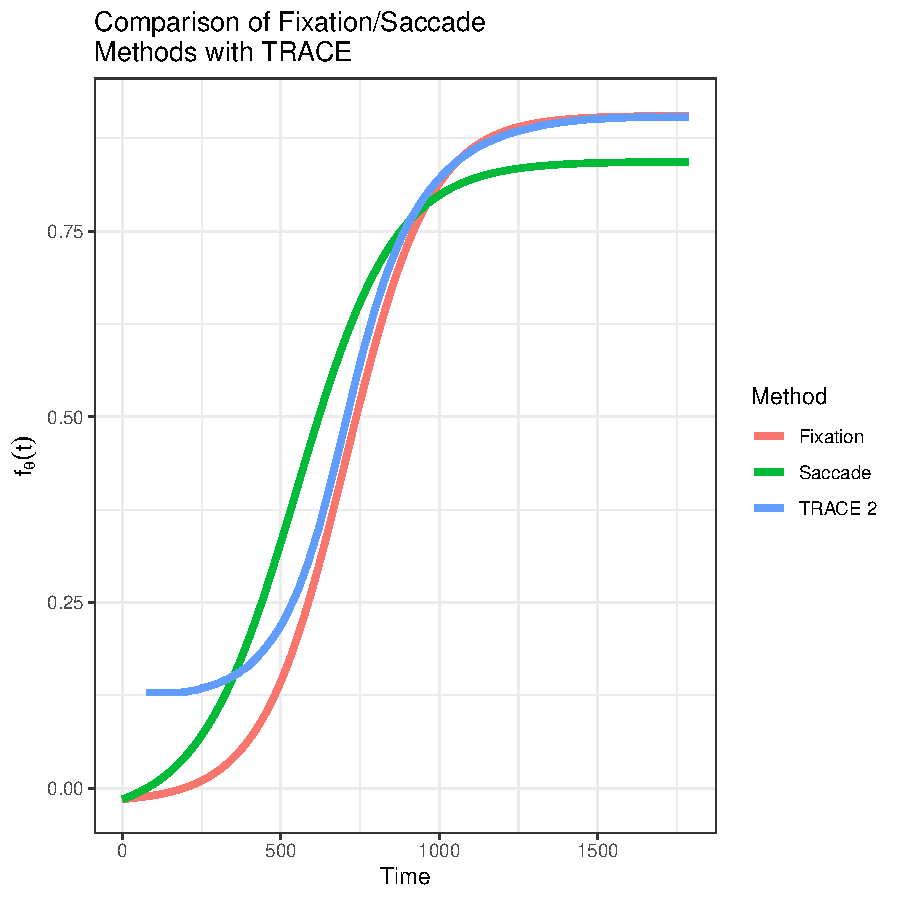
\includegraphics[width=0.45\textwidth]{sac_fix_trace_2.pdf}} 

    \caption{Examples of different temperatures used in LCR and how this effects TRACE activation. In (a), this leads to greater consistency with the saccade curve; in (b), with the fixation curve. This is evidenced also by RMS error values}
\label{fig:shades_of_trace2}
\end{figure}

%\begin{figure}[H]
%\centering
%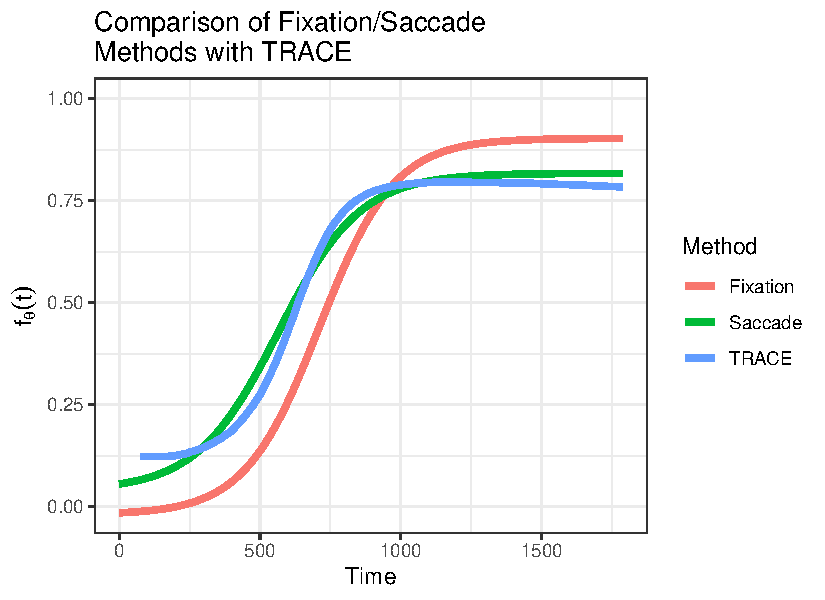
\includegraphics{sac_fix_trace_compare.pdf}
%\caption{this is just the mean value of the curve parameters. also only includes NH subjects. I feel like confidence intervals would make this chart look messy so might just instead include table of mean integrated squared error using approxfun since trace only has 108 data points and need a function to integrate in R}
%\end{figure}

Presented in Table~\ref{tab:mise_trace} is a summary of the RMS error of the 1000s simulations using both the saccade and fixation methods against two instantiations of TRACE. As we see and corresponding to (a) in Figure~\ref{fig:shades_of_trace2} we have better agreement between the saccade method and trace predictions; this relation is flipped for case (b). 


% latex table generated in R 4.2.2 by xtable 1.8-4 package
% Wed Jan 18 18:41:24 2023
\begin{table}[ht]
\centering
\begin{tabular}{rllrrrrrr}
  \hline
 & Method & TRACE & Min. & 1st Qu. & Median & Mean & 3rd Qu. & Max. \\ 
  \hline
1 & Proportion of Fixation & TRACE1 & 0.1148 & 0.1743 & 0.2181 & 0.2226 & 0.2583 & 0.4407 \\ 
  2 & Look Onset & TRACE1 & 0.0749 & 0.1051 & 0.1396 & 0.1449 & 0.1655 & 0.2933 \\ 
  3 & Proportion of Fixation & TRACE2 & 0.0991 & 0.1270 & 0.1529 & 0.1606 & 0.1712 & 0.3875 \\ 
  4 & Look Onset & TRACE2 & 0.0957 & 0.1404 & 0.1830 & 0.1879 & 0.2275 & 0.3734 \\ 
   \hline
\end{tabular}
\caption{Summary of RMS of two transformations of TRACE against saccade and fixation method}
\label{tab:mise_trace}
\end{table}

As an aside, this also lends itself to the idea of having a \textit{distribution} of curves associated with lexical activation rather than pursuing point estimation.  In some sense, this allows a natural way to account for the observed variability in experimental conditions without having to attempt to model it. Not sure if this is an idea worth elaborating on.

